\section{Konzept}

\begin{figure}[H]
  \begin{center}
    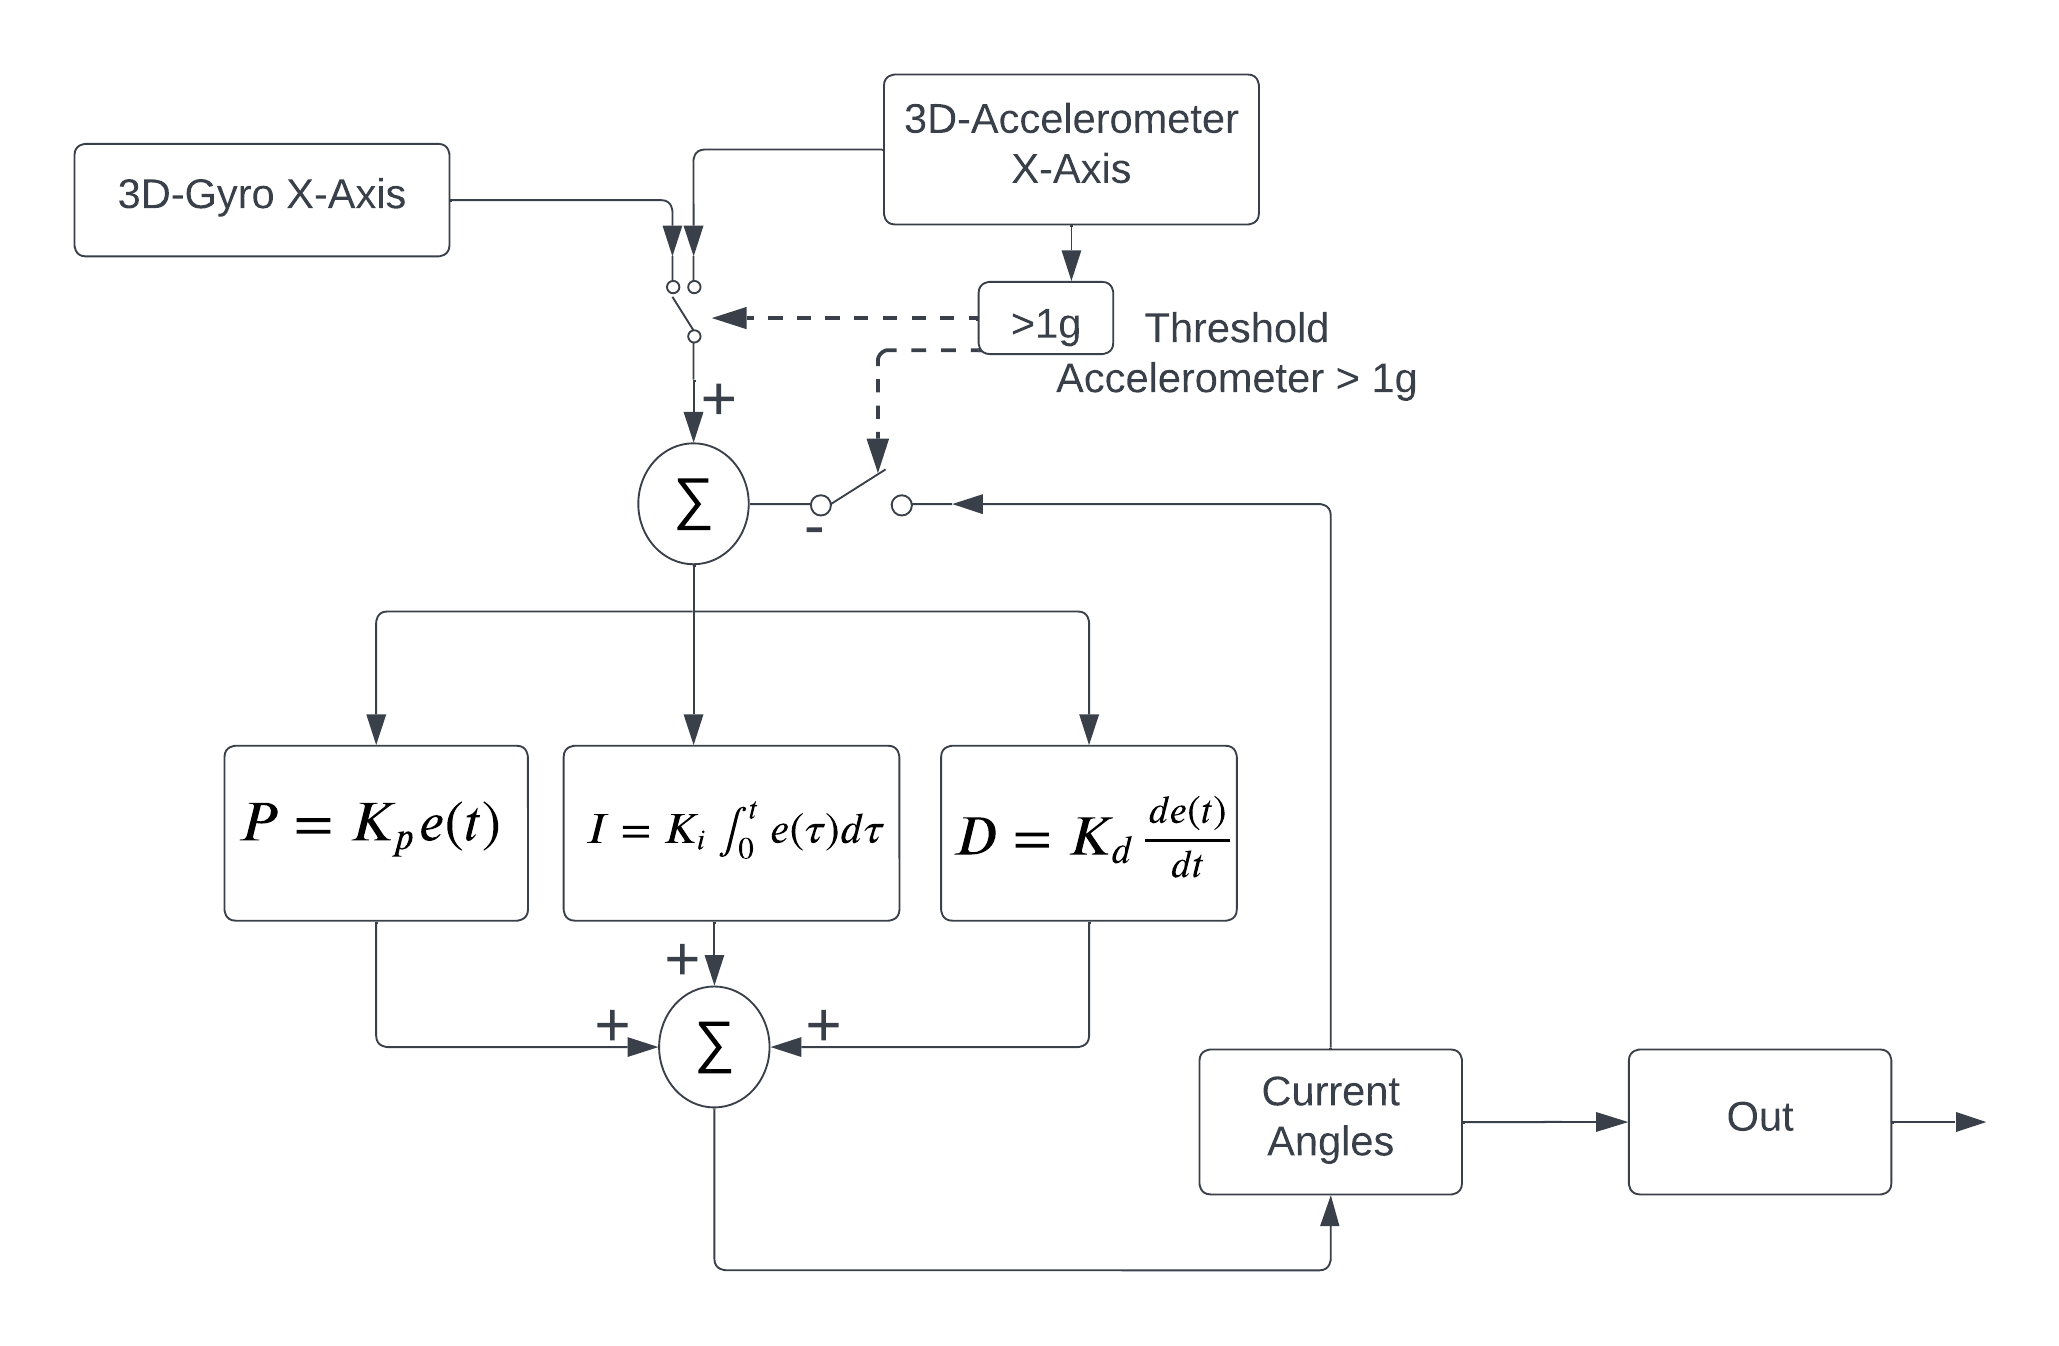
\includegraphics[width=1\linewidth]{content/images/PID_Loop.png}
    \caption{PID Loop}
  \end{center}
\end{figure}

\subsection{UseCase}
\begin{figure}[H]
  \begin{center}
    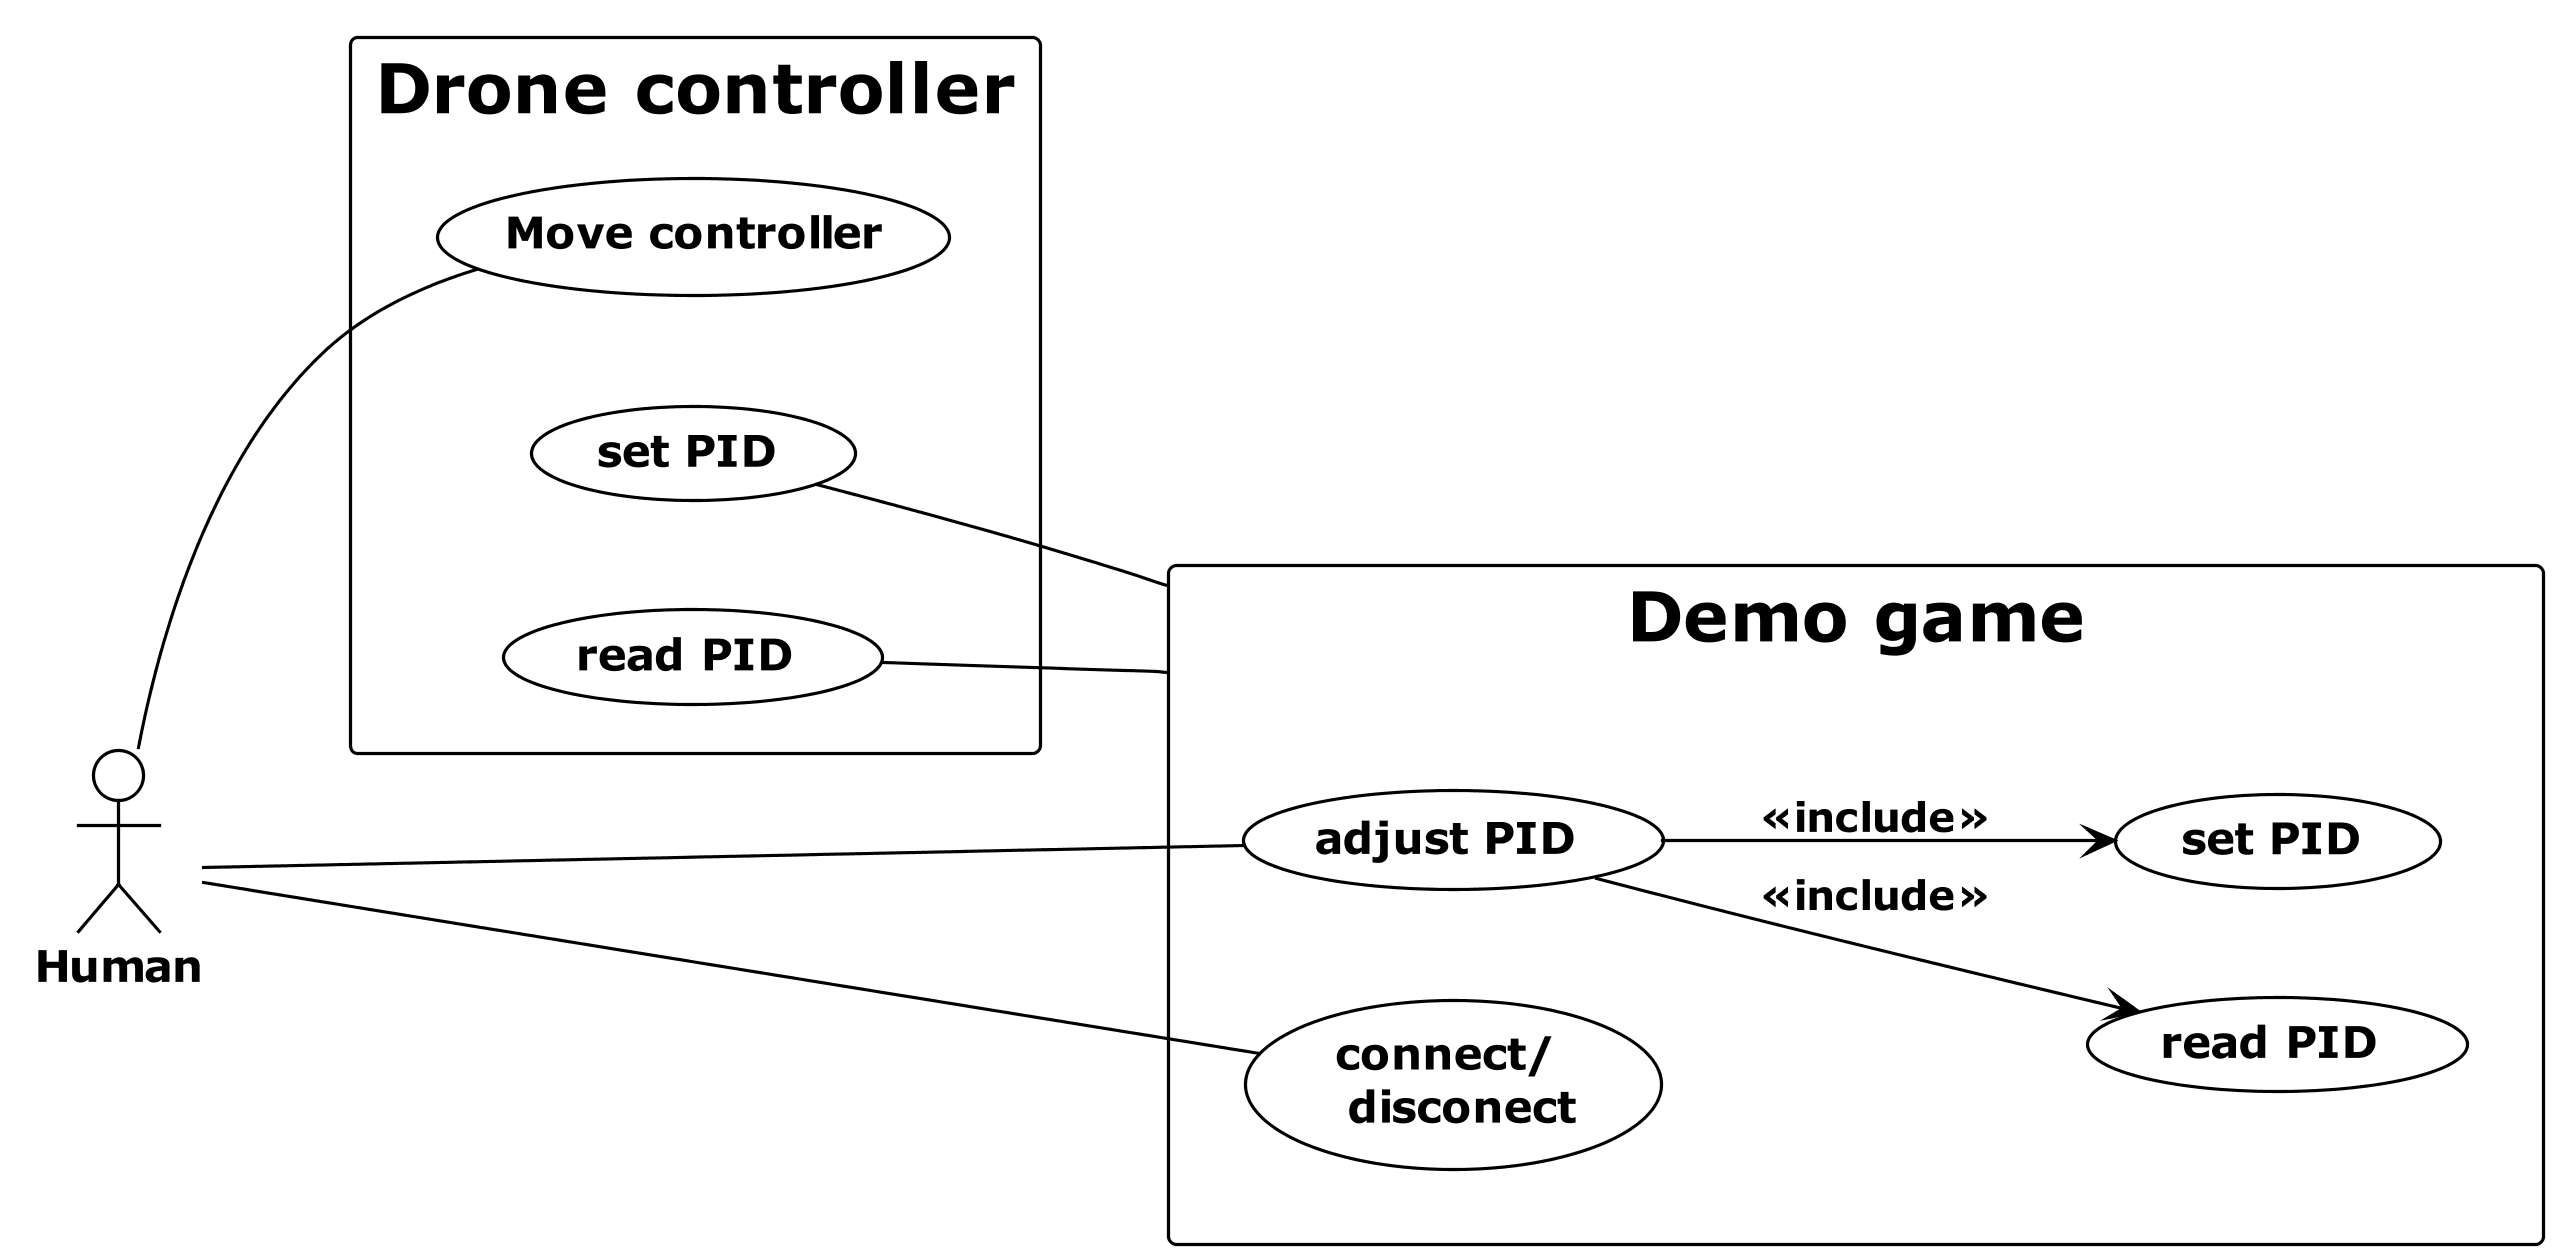
\includegraphics[width=0.9\linewidth]{content/diagrams/out/usecase/sendAngles.png}
    \caption{Send angles}
  \end{center}
\end{figure}

\subsection{Sequenzdiagramme}
\begin{figure}[H]
  \begin{center}
    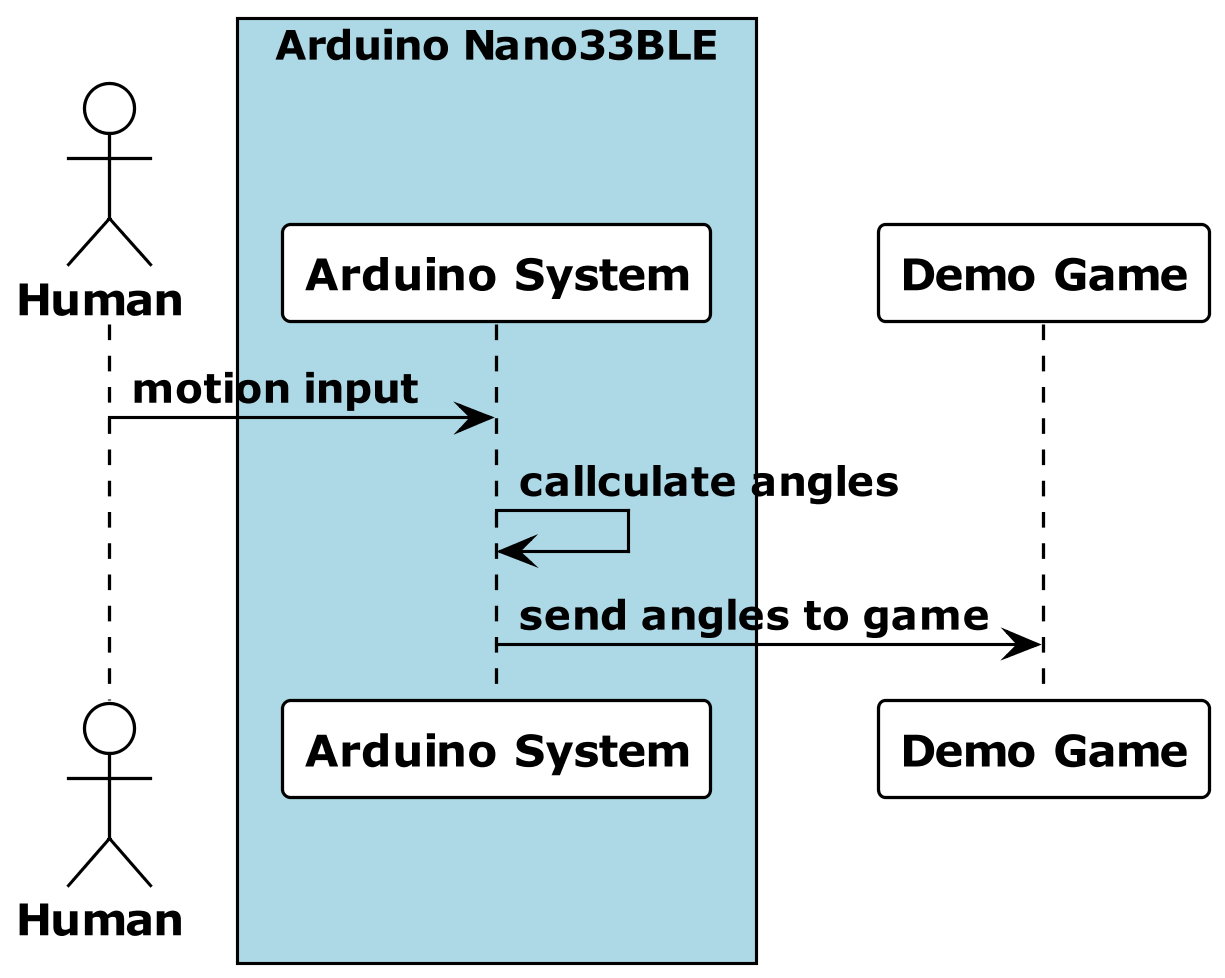
\includegraphics[width=0.7\linewidth]{content/diagrams/out/sequence/system.png}
    \caption{System}
  \end{center}
\end{figure}

\begin{figure}[H]
  \begin{center}
    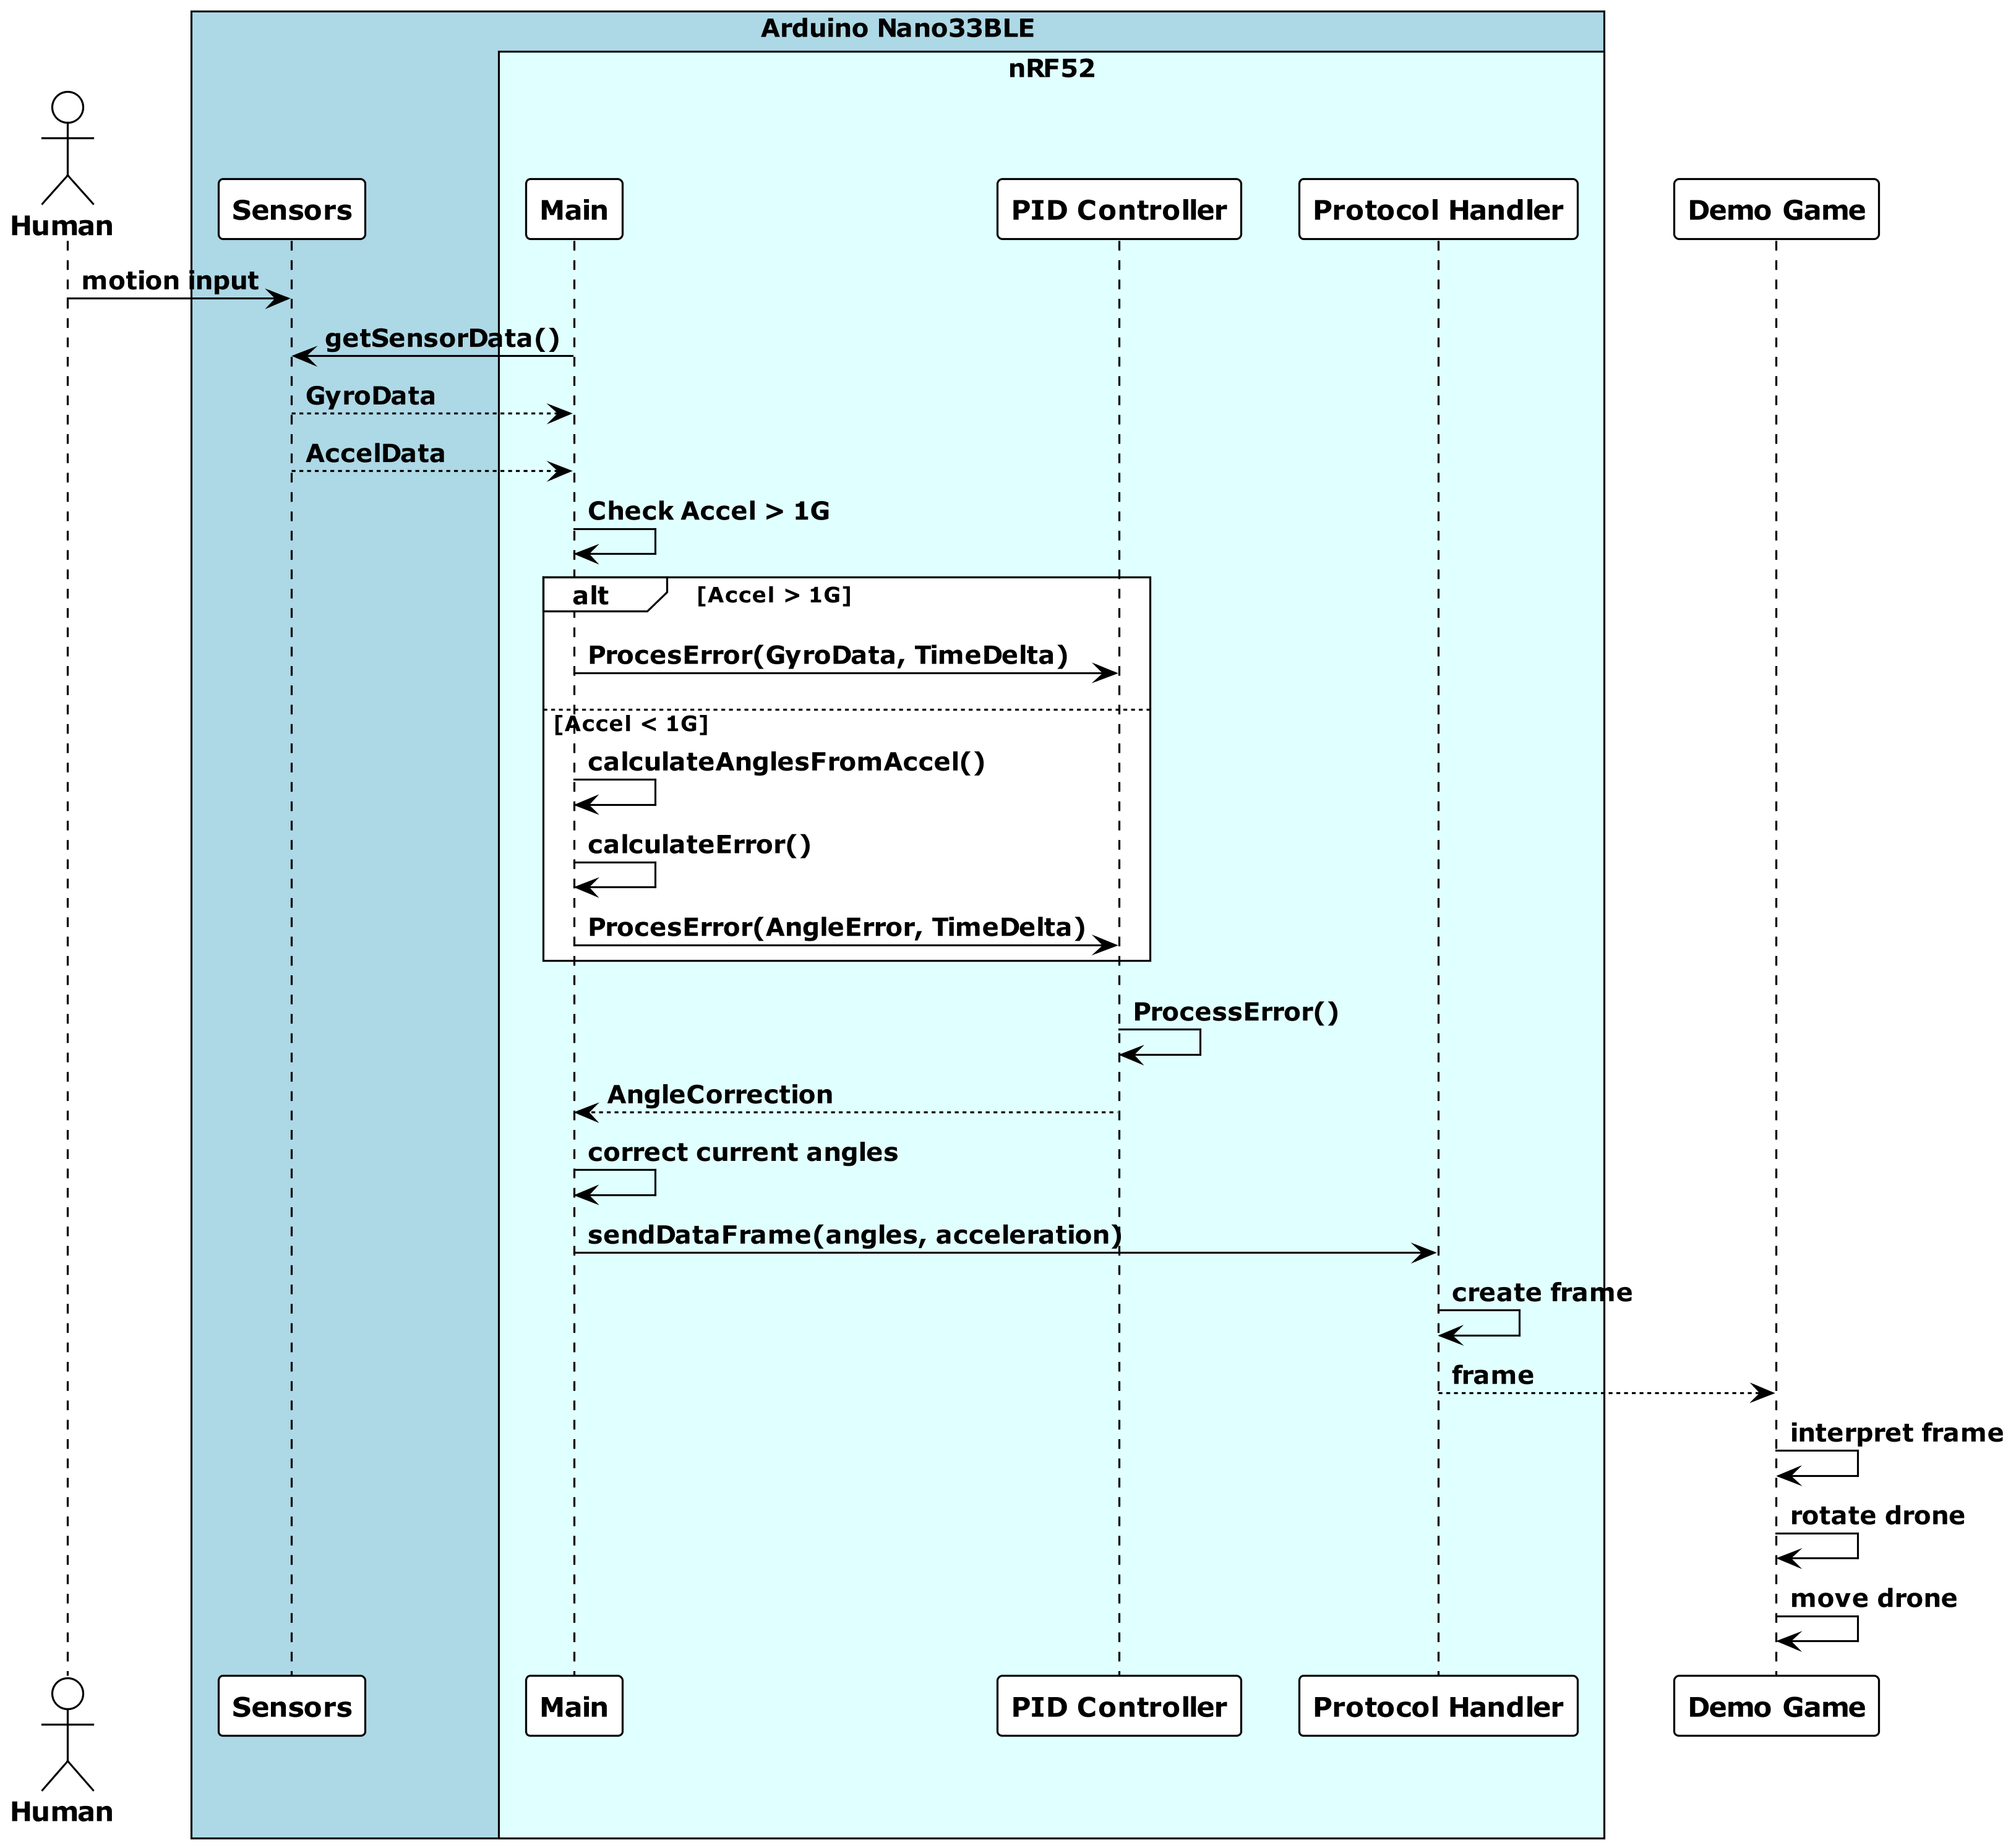
\includegraphics[width=1\linewidth]{content/diagrams/out/sequence/moveController.png}
    \caption{Move controller}
  \end{center}
\end{figure}

\subsection{Klassendiagramm}
\begin{figure}[H]
  \begin{center}
    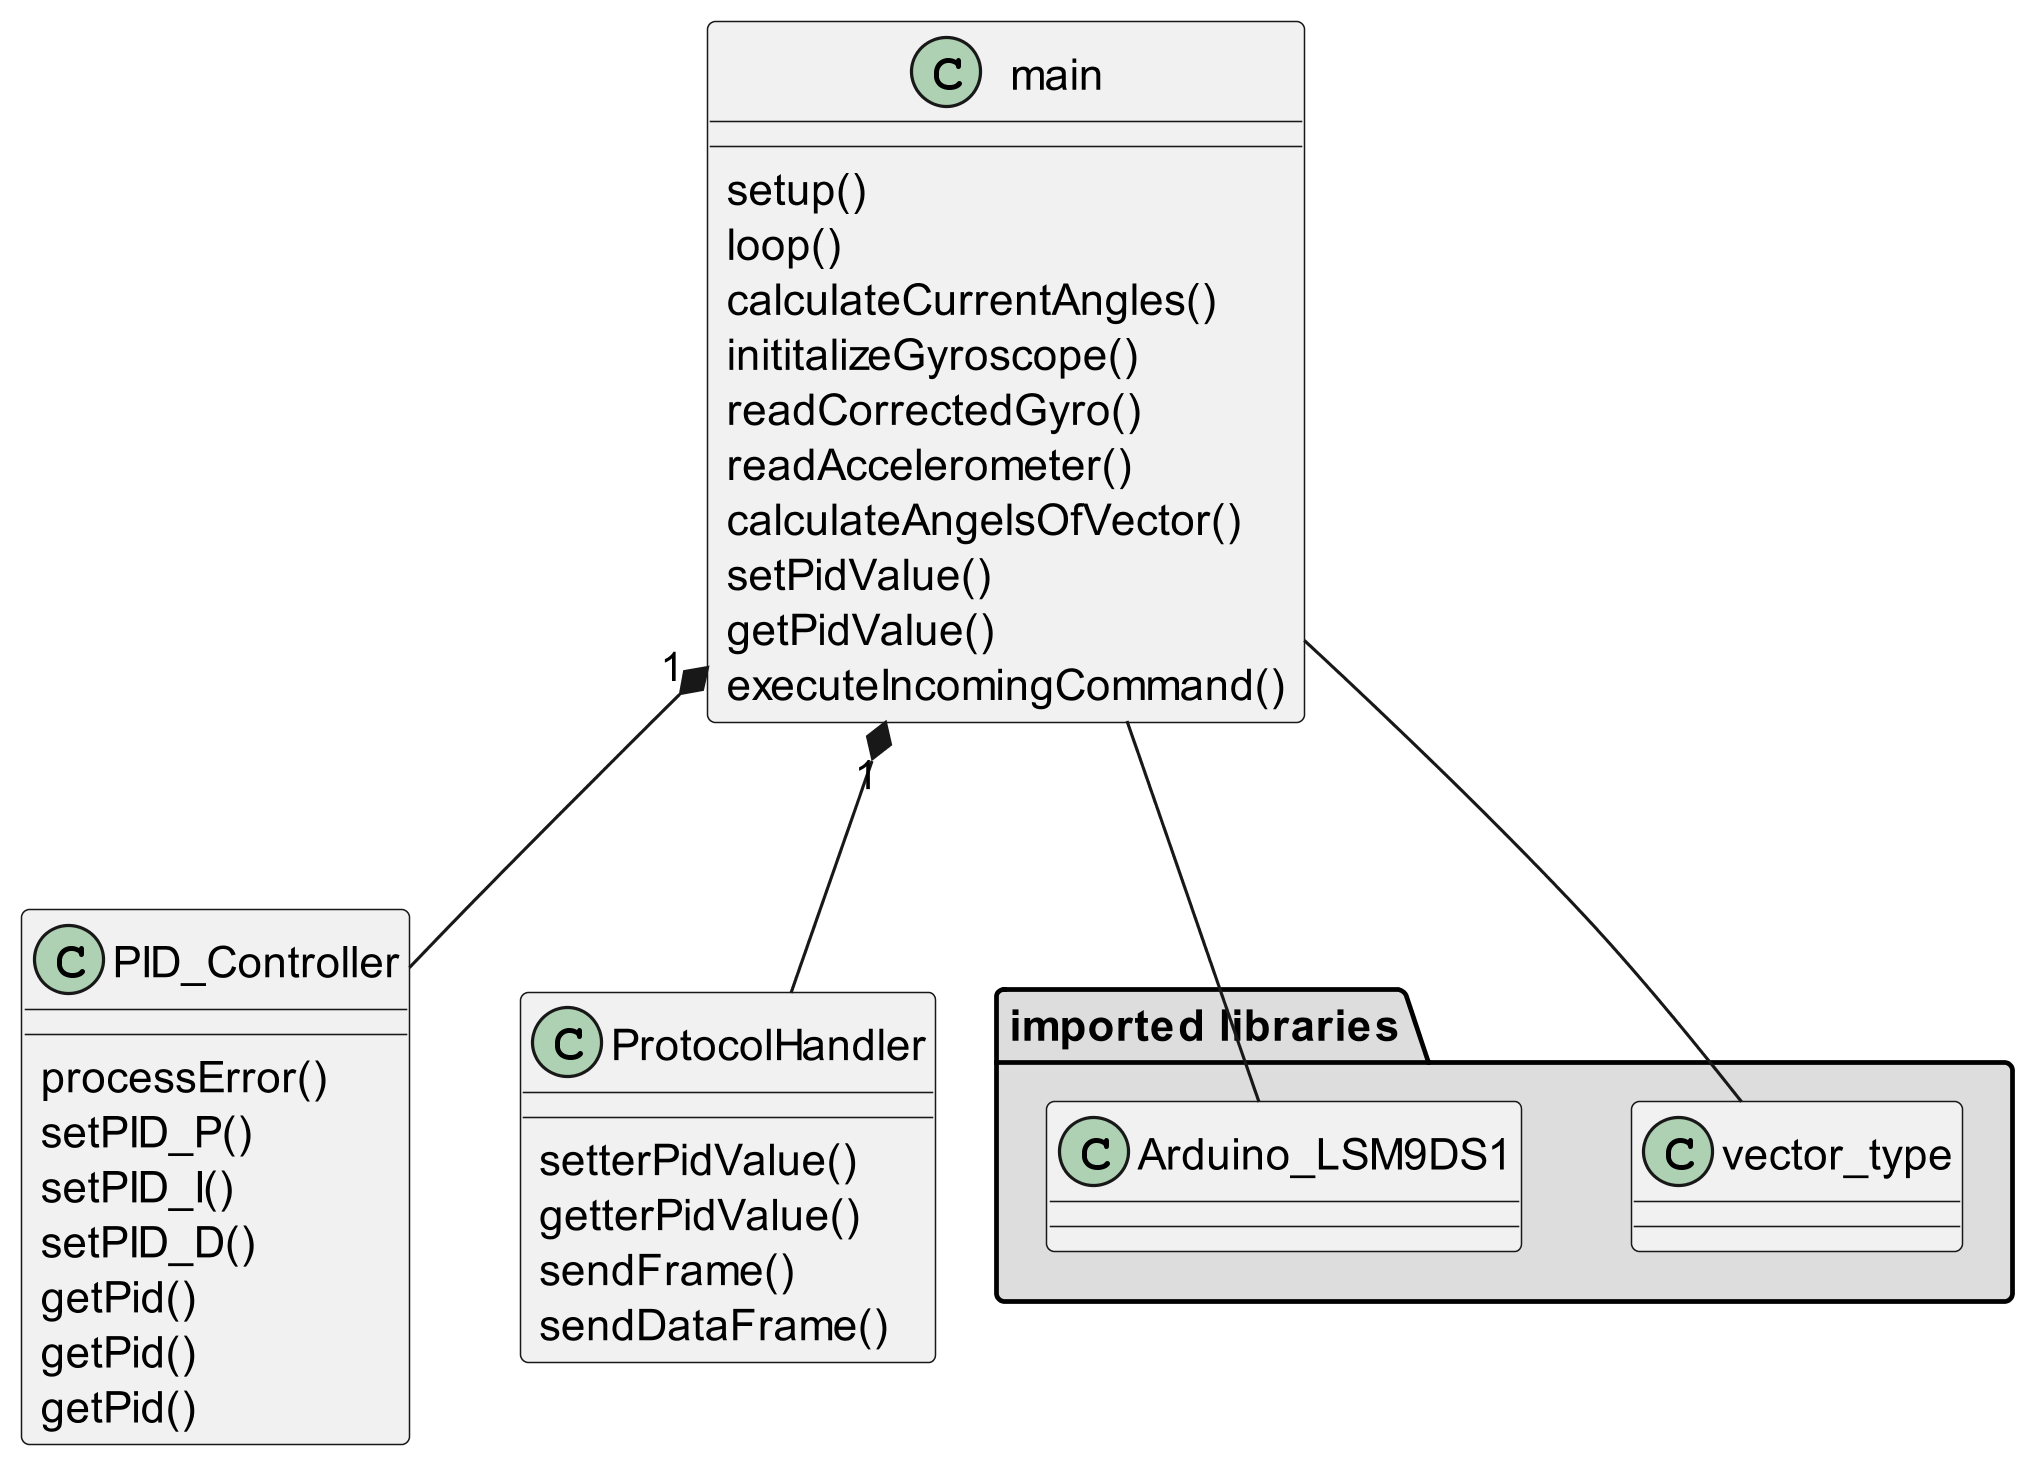
\includegraphics[width=0.8\linewidth]{content/diagrams/out/class/classdiagram.png}
    \caption{Klassendiagramm}
  \end{center}
\end{figure}

\subsection{Beschreibung der Klassen}
In diesem Kapitel werden die benutzten Klassen und deren Funktion kurz beschrieben.
\subsubsection{''main'' Klasse}
Die ''main'' Klasse ist die hauptklasse welche alle anderen Klassen Importiert. Hier befindet sich ebenfalls die setup() Funktion und die loop() Funktion welche vom Arduinosystem vorgeben sind.

\begin{table}[H]
  \centering
  \settowidth\tymin{executeIncomingCommand()}
  \setlength\extrarowheight{2pt}
  \begin{tabulary}{1.0\textwidth}{|L|L|}
    \hline
    \textbf{Klasse} &
    \textbf{Beschreibung}\\
    \hline
    setup() &
    Setupfunktion des Arduino. Wird ausgeführt wenn der Arduino gestartet wird.\\
    \hline
    loop() &
    Sie ist eine Endlosschleife, die nach jedem Durchlauf erneut aufgerufen wird.\\
    \hline
    initializeGyroscope() &
    Mit dieser Funktion wird das Gyroskop beim einschalten initialisiert und kalibriert.\\
    \hline
    calculateCurrentAngles() &
    \\
    \hline
    readCorrectetGyro() &
    \\
    \hline
    readAcceletometer() &
    \\
    \hline
    calculateAnglesOfVector() &
    \\
    \hline
    executeIncomingCommand() &
    Diese Funktion wertet den eingegangenen Befehl aus und führt anschliessend die entsprechende Funktion aus.\\
    \hline
    setPidValue() &
    Wird aus executeIncomingCommand() aufgerufen und setzt die eingegangenen PID-Werte über den PID Controller.\\
    \hline
    getPidValue() &
    Wird aus executeIncomingCommand() aufgerufen und sendet die angeforderten PID Werte zurück.\\
    \hline
  \end{tabulary}
  \caption{Beschreibung der ''main'' Klasse}
\end{table}

\subsubsection{PID Controller}

\subsubsection{ProtocolHandler}
